%%
%%
\documentclass[12pt]{book}
\usepackage{amsfonts,amssymb,amsmath,amsthm}
\usepackage{graphicx}
\usepackage{hyperref}
\usepackage{boxedminipage}
\usepackage{geometry}
\usepackage{array}
\usepackage{enumitem}


\newcolumntype{C}[1]{>{\centering\let\newline\\\arraybackslash\hspace{0pt}}m{#1}}

\setlength{\textheight}{10in}
\setlength{\textwidth}{7.4in}
\setlength{\topmargin}{-0.75in}
\setlength{\oddsidemargin}{-0.5in}
\setlength{\evensidemargin}{-0.5in}
\setlength{\parskip}{0.15in}
\setlength{\parindent}{0in}

\newenvironment{amatrix}[1]{%
  \left(\begin{array}{@{}*{#1}{c}|c@{}}
}{%
  \end{array}\right)
}


\begin{document}


\vspace{-1.0in}\begin{center}
\Large{MCV4U : Calculus and Vectors}\\
\Large{MCV4UR : Advanced Placement Calculus and Vectors }

\Large{Assignment \#3}


\end{center}

%\medskip

\vspace{0.015in}\hrulefill\ 

\textbf{Reference Declaration} %  Fill in your Reference Declarations in this section before your submit your assignment.

Complete the Reference Declaration section below in order for your assigment to be graded.

If you used any references beyond the course text and lectures (such as other texts, discussions with colleagues or online resources), indicate this information in the space below.  If you did not use any aids, state this in the space provided. 

Be sure to cite appropriate theorems throughout your work. You may use shorthand for well-known theorems like the FT, RRT, MVT, IVT, etc. 

Note: Your submitted work must be \textbf{your original work}. 

Family Name: Wong\\%Family Name Here
First Name: Max%First Name Here

Declared References: 
Geogebra for visualizing\\
Wolframalpha for \textbf{checking} answers
% Type your references here.
% You can use as many lines as required.

\vspace{0.015in}\hrulefill\ 

\newpage

% INSTRUCTIONS SECTION
\section*{Instructions}

\begin{center}
\setlength{\fboxrule}{2pt}
\begin{boxedminipage}{6.5in}
1.	Organize and express complete, effective and concise responses to each problem.\\
2.	Use appropriate mathematical conventions and notation wherever possible.\\
3.	Provide logical reasoning for your arguments and cite any relevant theorems. \\
4.  The quality of your communication will be heavily weighted.
\end{boxedminipage}
\end{center} 

% EVALUATION SECTION
\section*{Evaluation}

% LEARNING EXPECTATION(S)
\begin{itemize}
\item Students will demonstrate an understanding of derivative rules and use them to solve problems.
\end{itemize}

% RUBRIC
\begin{tabular}{| C{2in} | C{1in} | C{1in} | C{1in} | C{1in} |}
\hline
\textbf{Criteria} & \textbf{Level 1} & \textbf{Level 2} & \textbf{Level 3} & \textbf{Level 4} \\
\hline
\emph{Understanding of Mathematical Concepts} & Demonstrates limited understanding & Demonstrates some understanding & Demonstrates considerable understanding & Demonstrates thorough understanding of concepts \\
\hline
\emph{Selecting Tools and Strategies} & Selects and applies appropriate tools and strategies, with major errors, omissions, or mis-sequencing & Selects and applies appropriate tools and strategies, with minor errors, omissions, or mis-sequencing & Selects and applies appropriate tools and strategies accurately, and in a logical sequence & Selects and applies appropriate and efficient tools and strategies accurately to create mathematically elegant solutions \\
\hline
\emph{Reasoning and Proving} & Inconsistently or erroneously employs logic to develop and defend statements & Statements are developed and defended with some omissions or leaps in logic & Frequently develops and defends statements with reasonable logical justification & Consistently develops and defends statements with sophisticated and/or complete logical justification \\
\hline
\emph{Communicating} & Expresses and organizes mathematical thinking with limited effectiveness & Expresses and organizes mathematical thinking with some effectiveness & Expresses and organizes mathematical thinking with considerable effectiveness & Expresses and organizes mathematical thinking with a high degree of effectiveness \\
\hline
\end{tabular}

\pagebreak


%%%%%%%%%%%% PROBLEMS START HERE

\begin{enumerate}

%% PROBLEM 1
\item Determine whether the following statements are True (T) or False (F).

\begin{enumerate}
\item If $\vec{u} \cdot \vec{v} = 0$ then either $\vec{u} = \vec{0}$ or $\vec{v} = \vec{0}$.
\item $(\vec{u} \cdot \vec{v})\vec{u} \times (\vec{u} \times \vec{v})$ is a meaningful expression.
\item Force and velocity are scalar quantities.
\item If $|\vec{a}| = 1$ then $\vec{a}$ is a unit vector.
\item If $\vec{a} = \vec{b} \times \vec{c}$ and $\vec{a}$ is perpendicular to both $\vec{b}$ and $\vec{c}$, then $\vec{b}$ and $\vec{c}$ are collinear.
\item $\left\{ \vec{i}, \left(\begin{smallmatrix} 0 \\ 1 \\ 0 \end{smallmatrix}\right), \vec{i} \times \vec{j}\right\}$ is a spanning set of $\mathbb{R}^3$.
\item Given the standard basis vectors $\vec{i}, \vec{j}, \vec{k} \in \mathbb{R}^3$, we can express $\vec{k}$  as a linear combination of $\vec{i}$ and $\vec{j}$. 
\item If $\vec{a}$ and $\vec{b}$ are opposite vectors and $|\vec{a}| = n$ then $|\vec{b}| = -n$.
\item $\forall \vec{a}, \vec{b} \in \mathbb{R}^3$, $\vec{a} \times \vec{b} = \vec{b} \times \vec{a}$.
\item $\exists \vec{a}, \vec{b} \in \mathbb{R}^3$, $\vec{a} \times \vec{b} = \vec{b} \times \vec{a}$.
\item If $\forall m,n \in \mathbb{R}$, $|m\vec{a}| = |n\vec{a}|$ then $\vec{a}=\vec{0}$.
\item Given $\vec{u}, \vec{v} \in \mathbb{R}^3$, if $|\vec{u}| = |\vec{v}| = 1$ then $|\vec{u} \times \vec{v}| = 1$.
\item $\forall \vec{a}, \vec{b}, \vec{c} \in \mathbb{R}^3$, $\vec{a} \times (\vec{b} \times \vec{c}) = (\vec{a} \times \vec{b}) \times \vec{c}$.
\item $\forall \vec{x}, \vec{y} \in \mathbb{R}^3$, $|\vec{x} \times \vec{y}| = |\vec{y} \times \vec{x}|$.
\item Given two lines in $\mathbb{R}^3$, $\ell_1$ and $\ell_2$, either $\ell_1 \parallel \ell_2$ or $\ell_1$ intersects $\ell_2$ at some point in $\mathbb{R}^3$.
\item If $\vec{x}, \vec{y} \in \mathbb{R}^3$ then $\textrm{Span}\{ \vec{x}, \vec{y}\}$ is a plane in $\mathbb{R}^3$.
\item If $\{ \vec{a}, \vec{b} \}$ spans $\mathbb{R}^2$ then $\{ \vec{a}, \vec{a}+\vec{b} \}$ spans $\mathbb{R}^2$.
\item If $\vec{p}$ is a scalar multiple of $\vec{q}$ then $\vec{x} = t \vec{p} + \vec{q}$ , $t \in \mathbb{R}$, is a line through the origin.
\item Given $\vec{a}, \vec{b}, \vec{c} \in \mathbb{R}^4$, if $\vec{a} \cdot \vec{b} = 0$ and $\vec{b} \cdot \vec{c} = 0$ then $\vec{a} \cdot \vec{c} = 0$. 
\item If $\left(\begin{smallmatrix} 1 \\ 1 \\ 1 \end{smallmatrix}\right)$ is a solution to a system of linear equations then $\left(\begin{smallmatrix} 2 \\ 2 \\ 2 \end{smallmatrix}\right)$ is also a solution. 
\end{enumerate}

\newpage

\section*{True-False Answers}

\begin{enumerate}
\item F
\item
\item F
\item T
\item F
\item T
\item T
\item F
\item F
\item T
\item F
\item F
\item F
\item T
\item F
\item T
\item
\item F
\item F
\item F
\end{enumerate}

%% I would recommend sandwiching your solution to every problem between the kind of structure I have provided below re: initial \vspace, the Solution: heading and the ending \vspace.
%\vspace{0.3cm} 
%\textbf{Solution:}\\
% Your solution starts here.
%\vspace{0.3cm}

\newpage

%% PROBLEM 2
\item An \textbf{orthogonal spanning set of $\mathbb{R}^3$} is a set of 3 non-zero vectors, all of which are orthogonal to each other and span $\mathbb{R}^3$. Given $\vec{a} = \left(\begin{smallmatrix} 1 \\ -1 \\ 2 \end{smallmatrix}\right)$, \textbf{determine} vectors $\vec{b}$ and $\vec{c}$ such that $\{\vec{a}, \vec{b}, \vec{c}\}$ is an orthogonal spanning set of $\mathbb{R}^3$. \textbf{Express} the vector $\vec{u}= \left(\begin{smallmatrix} 1 \\ 0 \\ 1 \end{smallmatrix}\right)$ as a linear combination of the vectors in this spanning set. 

\vspace{0.3cm} 
\textbf{Solution to question 2:}\\
 Your solution starts here.
\vspace{0.3cm}

\newpage

%% PROBLEM 3
\item In a methane molecule ($CH_4$), a carbon atom is surrounded by four hydrogen atoms. Assume that the hydrogen atoms are located in space at $A(0,0,0), B(1,1,0), C(1,0,1) \textrm{ and } D(0,1,1)$ and that the carbon atom is located at $E\left(\frac{1}{2},\frac{1}{2},\frac{1}{2}\right)$. \textbf{Determine} the \emph{bond angle}, the angle from some hydrogen atom to the carbon atom, to another hydrogen atom.

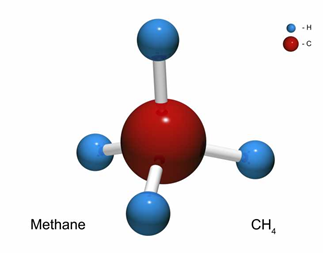
\includegraphics[scale=2]{Methane.png}

\vspace{0.3cm} 
\textbf{Solution to question 3:}\\
 Your solution starts here.
\vspace{0.3cm}


\newpage

%% PROBLEM 4
\item If $\theta$ is the acute angle between $\vec{a}$ and $\vec{b}$ then \textbf{prove} $proj_{\vec{a}}\vec{b} \cdot proj_{\vec{b}}\vec{a} = (\vec{a} \cdot \vec{b}) \cos^2(\theta)$.

\vspace{0.3cm} 
\textbf{Solution to question 4:}\\
 Your solution starts here.
\vspace{0.3cm}

\newpage

%% PROBLEM 5
\item \textbf{Determine} the equation of a line through the point $A(1,2,-3)$ and lying within the plane $x-2y+2z+9=0$.

\vspace{0.3cm} 
\textbf{Solution to question 5:}\\
 Your solution starts here.
\vspace{0.3cm}

\newpage

%% PROBLEM 8
\item \textbf{Determine} and \textbf{classify} the nature of the intersection between the following planes:
$$\Pi_1: x-5y+2z=10 $$
$$\Pi_2: x+7y-2z+6=0 $$
$$\Pi_3: 8x+5y+z=20 $$


\LaTeX{} note: You may find the \emph{amatrix} custom environment included in the code useful for creating the augmented matrix below.\\

$
\begin{amatrix}{3}
   1 & -5 & 2 & 10\\  1 & 7 & -2  & -6\\ 8 & 5 & 1 & 20 
 \end{amatrix}
$

\vspace{0.3cm} 
\textbf{Solution to question 8:}\\
 Your solution starts here.
\vspace{0.3cm}

%% $\equiv$ gives the "triple equal sign" equivalence relation if you want to use that for row equivalent matrices 

\newpage



\end{enumerate}
\end{document} 
